\section{Inserting Edges}
\label{sect:inserting-edges}

As clusters in our data set grow increasingly similar, we may want to indicate this similarity with new edges between existing clusters in the cluster graph. However, because the cluster graph is internally triangulated, we cannot insert any more edges on the inside of the graph. We can only insert edges in the outer face. Inserting an edge in the outer face is also only possible if it preserves the internal triangulatedness of the cluster graph. Inserting an edge $\{u,w\}$ in the outer face is therefore only permitted if $u$ and $w$ have a neighbor $v$ in common such that adding the edge forms a new triangular face with $v$. In case the outer face is bounded by exactly four vertices prior to inserting the edge $\{u,w\}$, it must be made explicit which of the resulting triangular faces is supposed to be the outer face. A valid edge insertion is illustrated in \cref{fig:insert-edge-outside-example}.

\begin{figure}[H]
	\centering
	\subfigure[]{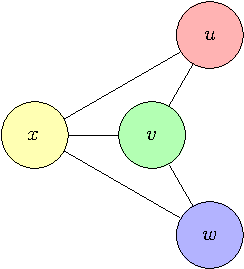
\includegraphics[height=29mm]{Resources/InsertEdgeOutside-Example-1.pdf}}
	\quad
	\subfigure[]{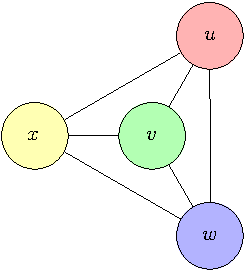
\includegraphics[height=29mm]{Resources/InsertEdgeOutside-Example-2.pdf}}
	\qquad
	\subfigure[]{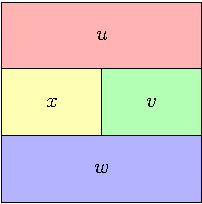
\includegraphics[height=29mm]{Resources/InsertEdgeOutside-Example-3.pdf}}
	\quad
	\subfigure[]{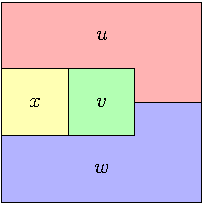
\includegraphics[height=29mm]{Resources/InsertEdgeOutside-Example-4.pdf}}
	\caption{A cluster graph and a polygonal dual thereof, before (a, b) and after (c, d) inserting the edge $\{u,w\}$ to form an internal triangular face with $v$.}
	\label{fig:insert-edge-outside-example}
\end{figure}

\lipsum
